\documentclass{article} % Defines the document class, article is commonly used
\usepackage[shortlabels]{enumitem}
\usepackage{amsmath}    % Allows for more advanced math formatting
\usepackage{amssymb}    % Provides additional mathematical symbols
\usepackage{amsthm}     % \qed
\usepackage{graphicx}   % image
\usepackage{float}      % image placement
\usepackage{hyperref}
\hypersetup{
    colorlinks=true,       % false: boxed links; true: colored links
    linkcolor=black,       % color of internal links
}
\usepackage[margin=1.5in]{geometry}
\usepackage{siunitx}

\begin{document}

\title{EEC133 Lab 3 Report}
\author{Tao Wang}
\date{\today}

\maketitle

\section*{Pre-lab}
\addcontentsline{toc}{section}{Pre-lab}
\textbf{Questions}
\begin{enumerate}[(1)]
    \item $W = 20 \si{mm}$. $L = 30 \si{mm}$.
    \item
    \item
    \item
          \begin{enumerate}[(a)]
              \item Return Loss from 2 to 3 GHz
                    \begin{figure}[H]
                        \centering
                        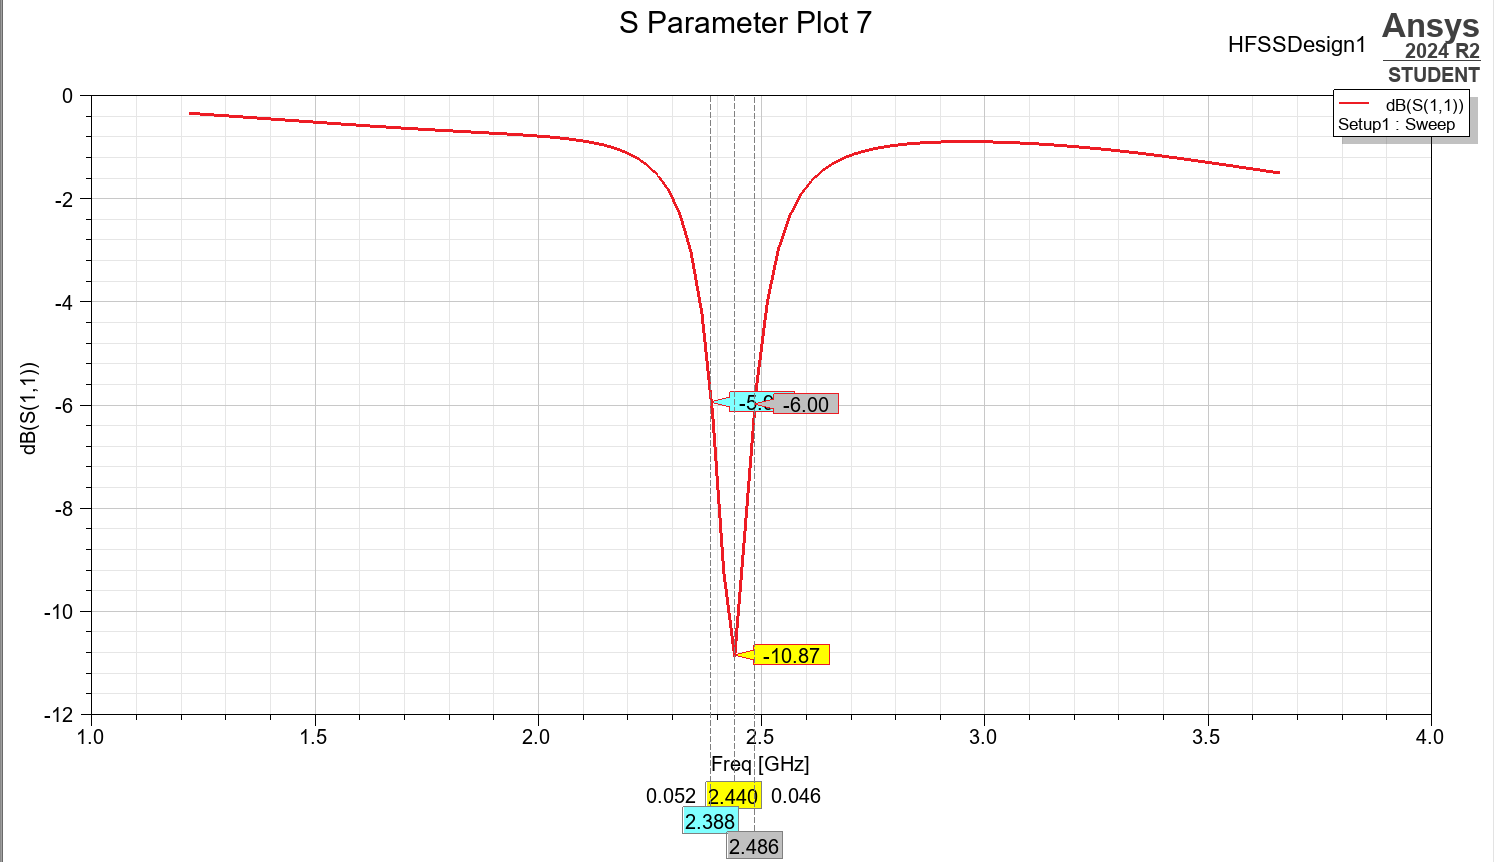
\includegraphics[width=0.7\textwidth]{./image/figure1.png}
                        \caption{$S_{1, 1}$ of Patch Antenna}
                    \end{figure}
              \item The bandwidth is in the range of 2.388 to 2.486 GHz. The antenna will work as a bluetooth antenna because the bandwidth is greater than the bluetooth bandwidth, 2.402-2.48 GHz.
              \item
          \end{enumerate}

\end{enumerate}




\end{document}
